\documentclass{ctexart}[UTF8]
\usepackage{dirtree}
\usepackage{listings}
\usepackage{xcolor}
\usepackage{graphicx}
\usepackage{enumerate}
\usepackage[a4paper]{geometry} 
\usepackage{amsmath,amsthm,mathtools,amssymb}
\usepackage{mathtools}
\usepackage{diagbox}
\usepackage{multirow,makecell}
\usepackage{float}
\usepackage{url}
\usepackage[nottoc]{tocbibind}
\usepackage{float}
\newcommand{\refe}[1]{Eq.\ref{#1}}
\newcommand{\reft}[1]{Theory.\ref{#1}\ }
\newcommand{\reff}[1]{图\ref{#1}\ }
\lstset{
 columns=fixed,
 numbers=left,                                        % 在左侧显示行号
 numberstyle=\tiny\color{gray},                       % 设定行号格式
 basicstyle=\small\ttfamily,
 frame=none,                                          % 不显示背景边框
 backgroundcolor=\color[RGB]{245,245,244},            % 设定背景颜色
 keywordstyle=\color[RGB]{40,40,255},                 % 设定关键字颜色
 numberstyle=\footnotesize\color{darkgray},           
 commentstyle=\color{gray}\ttfamily,                  % 设置代码注释的格式
 stringstyle=\rmfamily\slshape\color[RGB]{128,0,0},   % 设置字符串格式
 showstringspaces=false,
 breaklines=true,
 language=c++
}
\newtheorem{theorem}{Theory}[section]
\geometry{bottom=2cm,left=1cm,right=1cm}
\author{张配天-2018202180}
\title{上机7}
\begin{document}
    \maketitle
    \tableofcontents
    \clearpage
    \section{问题描述}
    实现矩阵链乘的备忘录算法。
    \subsection{输入}
    假设$k$个矩阵相乘,输入长度为$k+1$的矩阵规模序列,本题用课件例题进行测试,因此固定$k=6$;
    \subsection{输出}
    计算整个矩阵链的最小标量相乘次数;
    \section{算法思路}
    \begin{enumerate}
        \item 用两个二维数组$M$和$S$分别存储$A_i \dots A_j$相乘需要最少的标量乘法计算次数和最优划分位置;
        \item 递归调用Lookup\_Chain函数计算$A_i \dots A_k$和$A_{k+1} \dots A_{j}$的最少计算次数和最优划分位置;
        \item 如果遇到备忘录中已经存储的值,则直接$O(1)$查表;
    \end{enumerate}
    \section{复杂度分析}
    \begin{itemize}
        \item 第51行调用$\Theta(n^2)$次
        \item Lookup\_Chain函数的调用分为两类\begin{enumerate}[I.]
        
            \item \textbf{若$M[i][j] = \infty$执行16~38行;}第一种调用会发生$\Theta(n^2)$次,因为$M$一共有$\frac{n(n-1)}{2}$个表项,每次调用话费$O(n)$的时间;
            \item \textbf{否则,执行10~12行},此情况一定是被I.情况递归调用产生的,而每一次递归调用都会伴随$O(n)$次递归调用,因此有$O(n^3)$次调用,每次花费$O(1)$的时间,即查表;
        \end{enumerate}
    \end{itemize}
    \par 因此,算法总时间为$T(n) = \Theta(n^2)*O(n) + O(n^3) = O(n^3)$。
    \section{源代码}
    \begin{lstlisting}
#include<iostream>
#include<limits.h>
using namespace std;

// 备忘录法自顶向下实现动态规划
int Lookup_Chain(int **M,int ** S,int *p,int i,int j){
    
    // 如果值不是初始化的最大值,则返回
    // O(1)
    if(M[i][j] < INT_MAX){
        return M[i][j];
    }
    
    // 如果只有一个矩阵,直接返回0
    // O(1)
    if(i == j){
        return 0;
    }

    else
    {
        // 从i~j中选出一个最优的k
        // 最多只有n-1种情况,即子状态图中每个节点最多只有n-1条边
        for(int k = i;k < j;k++){

            // 计算不同k下Ai...Aj的总计算次数
            int q = Lookup_Chain(M,S,p,i,k) + Lookup_Chain(M,S,p,k+1,j) + p[i-1]*p[k]*p[j];

            // 如果有更优的,则直接替换备忘录中的值
            // 同时更新记录划分位置的矩阵
            if(q < M[i][j]){
                M[i][j] = q;
                S[i][j] = k;
            }
        }
    }
    // 返回Ai...Aj的最优计算次数
    return M[i][j];
}

// 初始化矩阵,调用算法计算最优计算次数
int Memoized(int ** S,int *p,int length){
    // 申请空间
    int ** M = new int*[7];
    for(int i = 1;i < length;i++){
        // 初始化两个数组,一个保存最优值,一个保存最优划分位置
        M[i] = new int[7]();
        S[i] = new int[7]();
        // 初始化为最大int
        for(int j = i;j < length;j++){
            M[i][j] = INT_MAX;
        }
    }
    return Lookup_Chain(M,S,p,1,length-1);
}

// 用于打印最终划分
void print_optimal(int ** s,int i,int j){
    if(i==j){
        cout<<"A"<<i;
    }
    else
    {
        cout<<'(';
        // 打印前半部分最优划分
        print_optimal(s,i,s[i][j]);
        // 打印后半部分最优划分
        print_optimal(s,s[i][j]+1,j);
        cout<<')';
    }
}

int main(){
    // 按照ppt输入矩阵规模序列
    int p[7] = {30,35,15,5,10,20,25};
    int ** S = new int*[7];
    cout<<"input the matrix scale sequence of LENGTH 6:"<<endl;
    for(int i = 0;i < 7;i++){
        cin>>p[i];
    }
    cout<<Memoized(S,p,7)<<endl;
    print_optimal(S,1,6);
    return 0;
}
    \end{lstlisting}
    \section{运行截图}
    \begin{figure}[H]
        \centering
        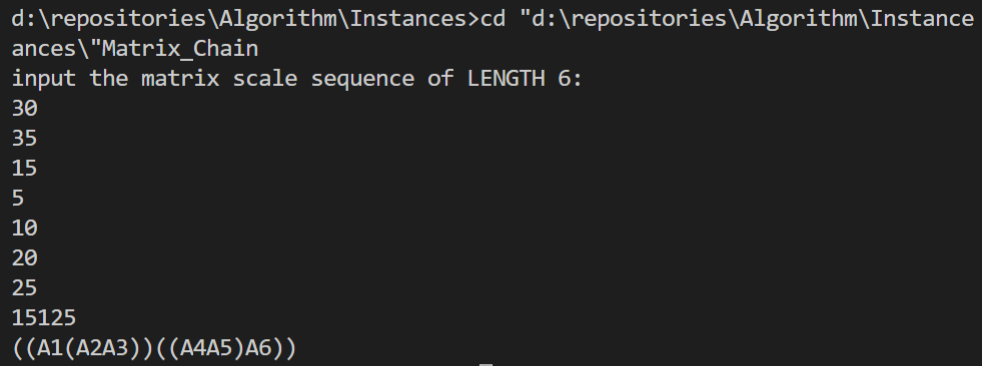
\includegraphics[width=12cm]{../Resources/7_1.png}
    \end{figure}
    和课件中结果一致。
\end{document}